\chapter{Desarrollo}
\section*{Introducci'on}

En 'este cap'itulo se muestra la arquitectura de los distintos esquemas de calendarizaci'on de trabajos en un entorno en la nube, para la implementaci'on de dichos esquemas se hace uso de un \textit{framework} llamado \textit{CloudSim}, el cual ser'a definido de igual manera.




\newpage
\addcontentsline{toc}{section}{Introducci'on}
\section{Aplicaci'on del marco metodol'ogico y de actividades de experimentaci'on}

En base de los dos primeros puntos descritos anteriormente en el marco metodol'ogico se realizar'on las siguientes actividades:

\begin{itemize}
	\item \textbf{Simular:} Se implementar'a a manera de simulaci'on un centro de datos con un entorno en la nube, las m'aquinas virtuales y el servidor inicializador que lo conforman.
	\item \textbf{Implementar:} En el centro de datos se desarrollar'an los algoritmos de calendarizaci'on que se mencionan con antelaci'on.
\end{itemize}

\subsection{Simulaci'on del Centro de Datos en la Nube}

 \textit{\textbf{Cloudsim}} es un nuevo, generalizado y extensible \textit{framework} de simulaci'on, que permite el modelaje, simulaci'on y experimentaci'on de infraestructuras emergentes de c'omputo en la nube y servicios de aplicaci'on (\citeauthor{calheiros2011cloudsim}, \citeyear{calheiros2011cloudsim}, p. 2).


\setcounter{figure}{2}
\renewcommand\thefigure{\arabic{figure}}
\begin{figure}[h!]
	\centering
	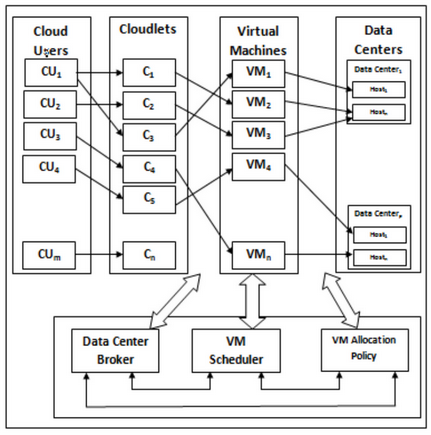
\includegraphics[scale=0.5]{media/imagenuno}
	\caption{Estilo de Trabajo de \textit{CloudSim}, Fuente: Chatterjee et al.}
	\label{fig:TrabajoCloudsim}	
\end{figure}


Entre los componentes que proporciona dicho \textit{framework} se encuentran los siguientes:

\begin{itemize}
	\item \textit{\textbf{Cloudlet:}} Esta clase modela las aplicaciones de servicio basadas en la nube como pueden ser env'io de contenido, redes sociales, y flujo de trabajo empresarial (\citeauthor{calheiros2011cloudsim}, \citeyear{calheiros2011cloudsim}, cap. 4).
	\item \textit{ \textbf{Datacenter:}} Esta clase modela el núcleo de los servicios en un nivel de infraestructura \textit{(hardware)} que son ofrecidos por \textit{Cloud Providers (Amazon, Azure, App Engine)}. Estos son encapsulados en un conjunto de \textit{host} que pueden ser homogéneos o heterogéneos con respecto a sus configuraciones de \textit{hardware} (memoria, n'ucleos, capacidad, y almacenamiento) (\citeauthor{calheiros2011cloudsim}, \citeyear{calheiros2011cloudsim}, cap. 4).
	\item \textit{ \textbf{DatacenterBroker:}} Esta clase modela un \textit{broker}, el cual es responsable de mediar las negociaciones entre el \textit{SaaS} y los \textit{Cloud providers}; y dichas negociaciones son manejadas por los requerimientos \textit{QoS} (\citeauthor{calheiros2011cloudsim}, \citeyear{calheiros2011cloudsim}, cap. 4).
	\item  \textit{\textbf{Host:}} Esta clase modela los recursos f'isicos como una computadora o un servidor de almacenamiento (\citeauthor{calheiros2011cloudsim}, \citeyear{calheiros2011cloudsim}, cap. 4).
	\item  \textit{\textbf{Vm:}} Esta clase modela una M'aquina Virtual \textit{(VM)}, la cual es administrada y hosteada por un componente \textit{host} en la nube. Cada \textit{VM} tiene acceso a un componente que almacena las siguientes características relacionadas a una \textit{VM}: memoria accesible, procesador, tama'no de almacenamiento (\citeauthor{calheiros2011cloudsim}, \citeyear{calheiros2011cloudsim}, cap. 4).
\end{itemize}


\newpage

\subsection{Implementaci'on de los Algoritmos}

Existen varios algoritmos para calendarizar los trabajos en el c'omputo en la nube. La mayor ventaja de estos algoritmos es obtener el mayor rendimiento. Los principales ejemplos de algoritmos de calendarizaci'on son: \textit{FCFS, Round Robin, Min-Min, Max-Min y algoritmos de meta heurísticas}  (\citeauthor{shimpy2014different}, \citeyear{shimpy2014different}, p. 1).



De los algoritmos mencionados anteriormente, se presentan los siguientes:


\begin{itemize}
	\item \textit{\textbf{FCFS:}} Ejecuta las tareas en orden de llegada, es decir, el primero en llegar es el primero en ser atendido.
	\item \textit{\textbf{Min-Min:}} Selecciona las tareas m'as pequeñas para ser ejecutadas primero.
	\item  \textit{\textbf{Max-Min:}} Selecciona las tareas m'as grandes para ser ejecutadas primero.
\end{itemize}

En un entorno de trabajo normal, la forma descrita anteriormente la podemos ver de la siguiente manera, Figura (\ref{fig:cuatro}):


%\setcounter{figure}{3}
\renewcommand\thefigure{\arabic{figure}}
\begin{figure}[H]
	\centering
	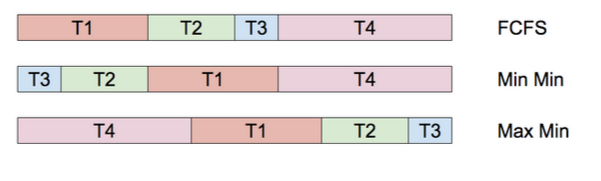
\includegraphics[scale=0.7]{media/imagendos}
	\caption{Esquema de trabajo de algoritmos de calendarizaci'on, Fuente: Elaboraci'on propia.}
	\label{fig:cuatro}
\end{figure}


Sin embargo en un entorno en la nube, al ser m'ultiples m'aquinas virtuales alojadas en distintos \textit{hosts}, que a su vez pueden formar parte de uno o m'as \textit{datacenters}, dicho esquema tiene que ser modificado para poder adoptar un estilo de trabajo similar al proporcionado por el \textit{framework}, por lo que los resultados quedan de la distinta manera:

\newpage

%\setcounter{figure}{4}
\renewcommand\thefigure{\arabic{figure}}
\begin{figure}[h!]
	\centering
	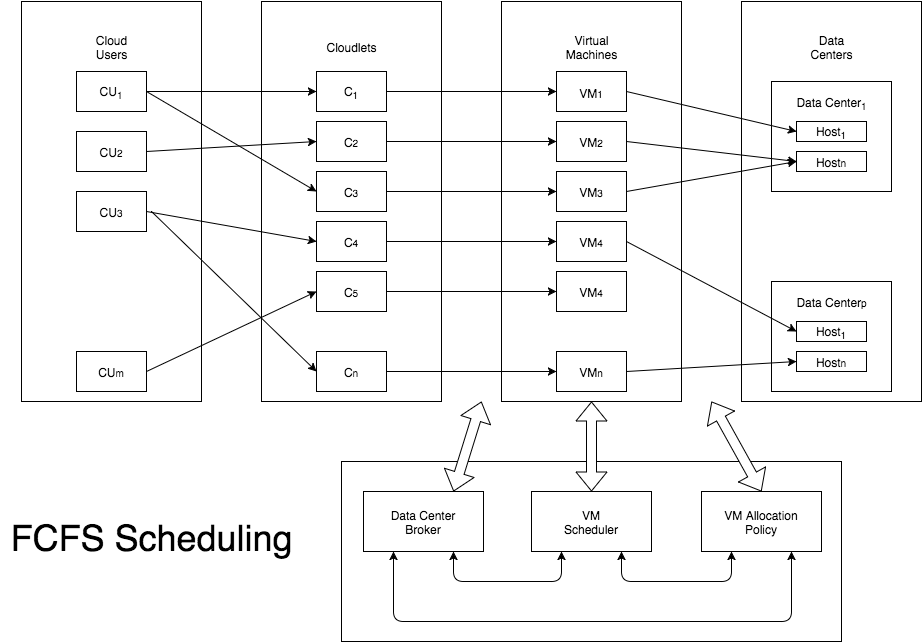
\includegraphics[scale=0.4]{media/imagentres}
	\caption{Arquitectura FCFS para un entorno en la nube. Fuente: Elaboraci'on propia.}
	\label{fig:fcfs}
\end{figure}

Como podemos apreciar en el diagrama (Figura \ref{fig:fcfs}), podemos tener \emph{m} usuarios ejecutando \emph{n} tareas, sin embargo la asignaci'on de m'aquinas virtuales va dependiendo del orden de llegada de dichas tareas, y quien se encarga de repartir las tareas es el \textit{datacenterBroker}.
\newpage

De manera similar tenemos los siguientes algoritmos \textit{Min-Min} (Figura: \ref{fig:min}) y \textit{Max-Min} (Figura: \ref{fig:max}):

%\setcounter{figure}{5}
\renewcommand\thefigure{\arabic{figure}}
\begin{figure}[h!]
	\centering
	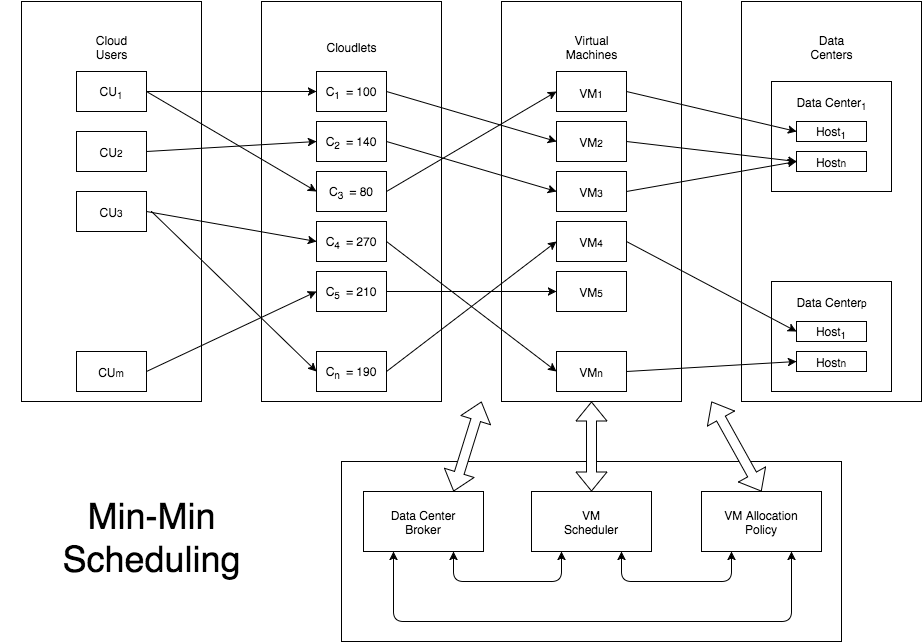
\includegraphics[scale=0.4]{media/imagencinco}
	\caption{Arquitectura de \textit{Min-Min} para un entorno en la nube. Fuente: Elaboraci'on propia.}
	\label{fig:min}
\end{figure}

Para el algoritmo de \textit{Min-Min} (Figura: \ref{fig:min}) obtenemos la lista de tareas, a partir de la informaci'on de ellas, procedemos a ordenarlas de menor a mayor tamaño asignando la de menor tamaño en la primera máquina virtual, la siguiente tarea de acuerdo al tamaño pasa a la segunda máquina y así sucesivamente.

\newpage
%\setcounter{figure}{6}
\renewcommand\thefigure{\arabic{figure}}
\begin{figure}[h!]
	\centering
	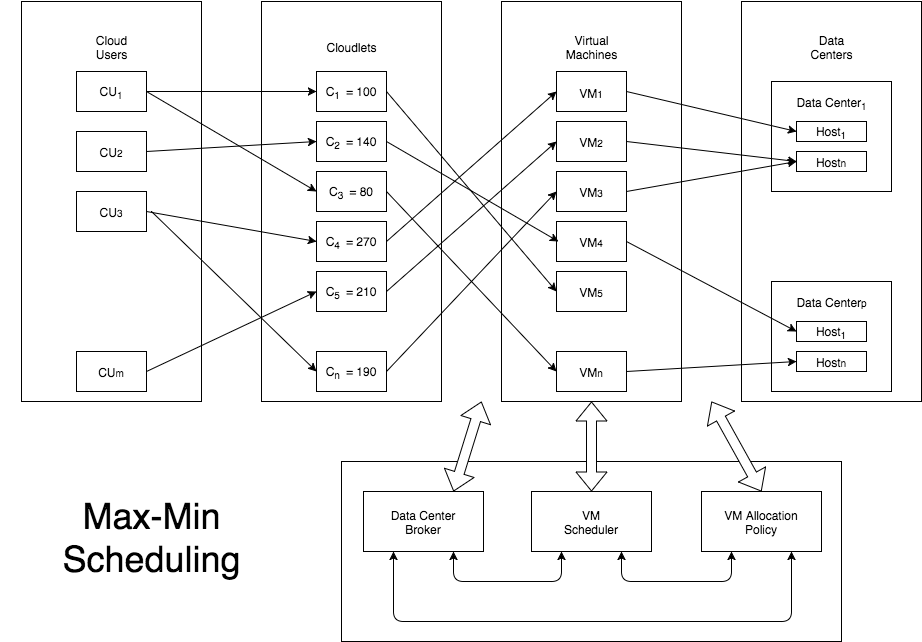
\includegraphics[scale=0.4]{media/imagencuatro}
	\caption{Arquitectura de \textit{Max-Min} para un entorno en la nube. Fuente: Elaboraci'on propia.}
	\label{fig:max}
\end{figure}

En la figura \ref{fig:max} tenemos el algoritmo de \textit{Max-Min} el cual ordena la lista de tareas de mayor a menor tamaño antes de asignarlas a las máquinas virtuales, una vez ordenada dicha lista procede a asignar la tarea más grande en la primera máquina, la siguiente en la segunda y así sucesivamente hasta terminar la asignación de las tareas.

\newpage 



Est'as son algunas capturas del c'odigo para la implementaci'on de los primeros algoritmos, el centro de datos:

\textbf{Configuración de Elementos del \textit{Datacenter} y \textit{DatacenterBrokers} para Algoritmos de Calendarización}
\addcontentsline{toc}{section}{Configuración de Elementos del Datacenter y DatacenterBrokers para Algoritmos de Calendarización}

%\setcounter{figure}{7}
\renewcommand\thefigure{\arabic{figure}}
\begin{figure}[h!]
	\centering
	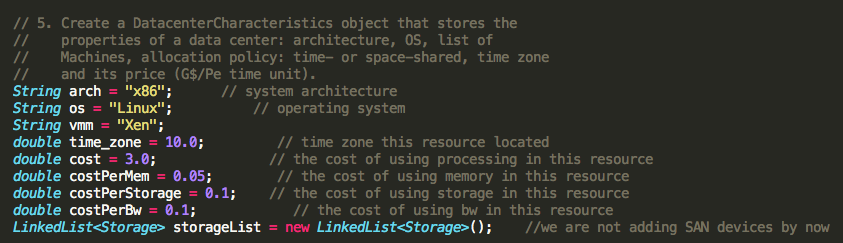
\includegraphics[scale=0.4]{media/caracteristicas_datacenter}
	\caption{Características del \textit{datacenter}. Fuente: Elaboración propia}
	\label{fig:DCar}
\end{figure}

Como paso inicial debemos de configurar las características que tendrá nuestro \textit{datacenter}, para eso tenemos que definir la arquitectura, el tipo de sistema operativo, costos de utilización de memoria, almacenamiento y ancho de banda, entre otros (Figura: \ref{fig:DCar}).

%\setcounter{figure}{8}
\renewcommand\thefigure{\arabic{figure}}
\begin{figure}[h!]
	\centering
	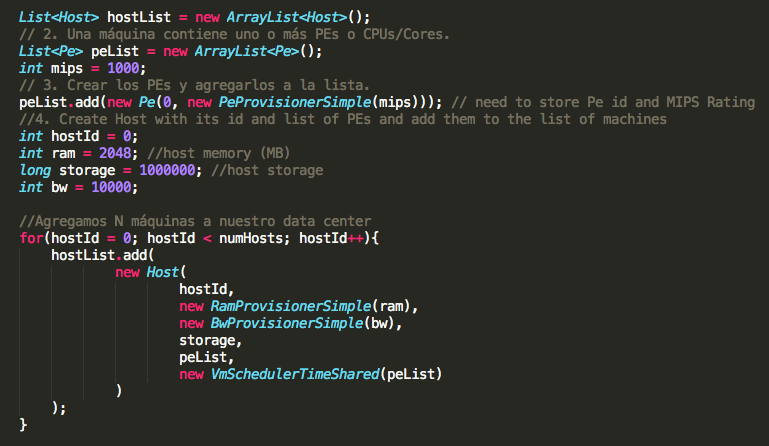
\includegraphics[scale=0.4]{media/caracteristicas_host}
	\label{fig:HCar}
	\caption{Características del \textit{Host}. Fuente: Elaboración propia}
\end{figure}

De igual manera tenemos que asignar las características que tendrá cada \textit{host} (Figura: \ref{fig:HCar}) dentro del datacenter, tales como el número de procesadores, número de instrucciones por segundo, memoria RAM, capacidad de almacenaiento y el ancho de banda.

%\setcounter{figure}{9}
\renewcommand\thefigure{\arabic{figure}}
\begin{figure}[h!]
	\centering
	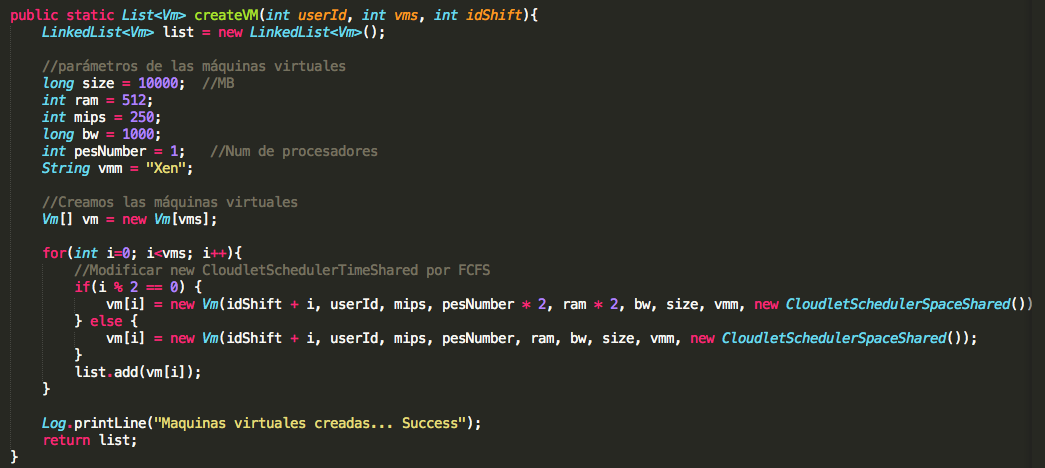
\includegraphics[scale=0.4]{media/creacion_vm}
	\caption{Características de las máquinas virtuales. Fuente: Elaboración propia}
	\label{fig:VCar}
\end{figure}

Continuando con las configuraciones, en la Figura \ref{fig:VCar} se muestran las utilizadas en las máquinas virtuales, las cuales son: Tamaño de la Imagen, Memoria Ram Virtual, Número de instrucciones por segundo, ancho de banda y el número de procesadores.

%\setcounter{figure}{10}
\renewcommand\thefigure{\arabic{figure}}
\begin{figure}[h!]
	\centering
	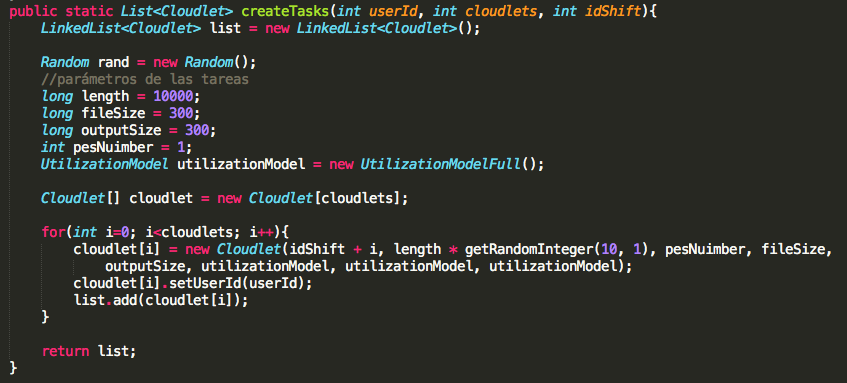
\includegraphics[scale=0.4]{media/creacion_cloudlet}
	\caption{Características de las Tareas \textit{(cloudlets)}. Fuente: Elaboración propia}
	\label{fig:TCar}
\end{figure} 

Además de los recursos, se debe de hacer la configuración de las tareas a simular (Figura: \ref{fig:TCar}), teniendo como parámetros el tamaño de la tarea, tamaño de entrada y de salida, así como el número de procesadores que ocupará la tarea, esto último refleja la complejidad de la tarea.


\newpage


\textbf{\textit{DatacenterBrokers} para Algoritmos de Calendarización}
\addcontentsline{toc}{section}{DatacenterBrokers para Algoritmos de Calendarización}

Partiendo del Esquema presentado en la figura: \ref{fig:TrabajoCloudsim} el trabajo presentado se lleva a cabo en la parte de Tareas (\textit{cloudlets}) y Máquinas Virtuales(\textit{Virtual Machines}) ya que se pretende mejorar un algoritmo de calendarización de tareas.
Para ello según muestra el diagrama, el encargado de asignar cada tarea en una máquina virtual es el \textit{datacenter broker}, el cual toma la lista de tareas así como la lista de máquinas virtuales, y de acuerdo a algún algoritmo realiza la asignación de cada una de las tareas en las distintas máquinas virtuales disponibles.

%\setcounter{figure}{11}
\renewcommand\thefigure{\arabic{figure}}
\begin{figure}[h!]
	\centering
	\includegraphics[scale=0.4]{media/FCFS_broker}
	\caption{\textit{FCFS Broker}. Fuente: Elaboración propia}
	\label{fig:fcfsBroker}
\end{figure}

La Figura: \ref{fig:fcfsBroker} muestra el algoritmo de FCFS, recorre la lista de tareas y la asigna en la máquina virtual correspondiente calculando la tarea actual $i$ en la máquina virtual $i\%reqVms$ donde $reqVms$ es el número de máquinas virtuales.

\newpage

En la Figura: \ref{fig:minminBroker} tenemos la implementación del algoritmo \textit{Min-Min} en el cual podemos apreciar el ordenamiento de la lista antes de pasar a  la asignación de las máquinas virtuales.

%\setcounter{figure}{12}
\renewcommand\thefigure{\arabic{figure}}
\begin{figure}[h!]
	\centering
	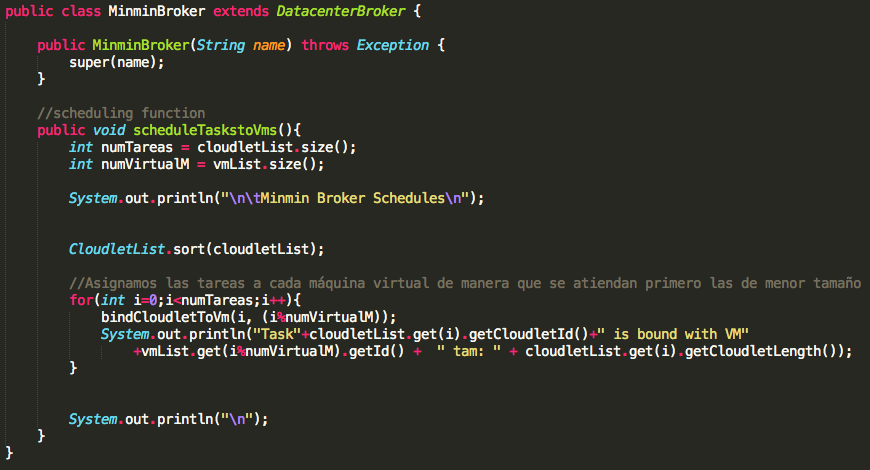
\includegraphics[scale=0.4]{media/minmin_broker}
	\caption{\textit{Min-Min Broker}. Fuente: Elaboración propia}
	\label{fig:minminBroker}
\end{figure}

En la Figura: \ref{fig:maxminBroker} observamos la implementación del algoritmo de \textit{Max-Min} el cual hace un ordenamiento de mayor a menor, véase la función \textbf{\textit{revert}} utilizada, la cual se explicará más adelante.

%\setcounter{figure}{13}
\renewcommand\thefigure{\arabic{figure}}
\begin{figure}[h!]
	\centering
	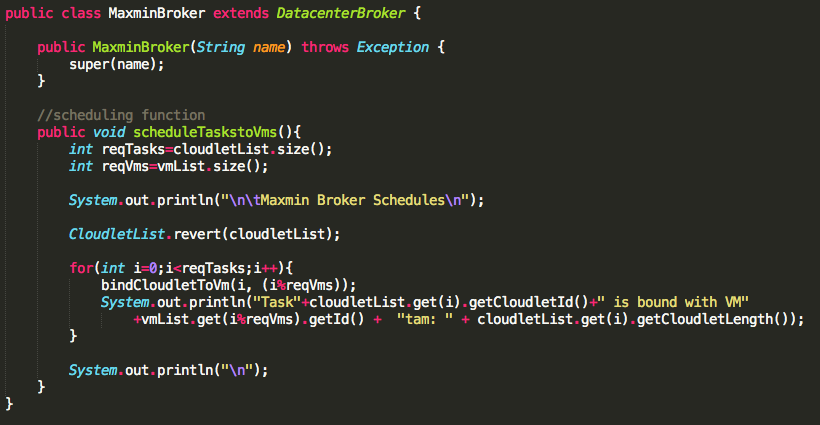
\includegraphics[scale=0.4]{media/maxmin_broker}
	\caption{\textit{Max-min Broker}. Fuente: Elaboración propia}
	\label{fig:maxminBroker}
\end{figure}

\newpage
En la Figura: \ref{fig:sortRevert} tenemos la implementación de los métodos de ordenamiento utilizados, el \textbf{sort} utilizado para ordenar las tareas de menor a mayor de acuerdo al tamaño y el \textbf{revert} de forma inversa.

%\setcounter{figure}{14}
\renewcommand\thefigure{\arabic{figure}}
\begin{figure}[h!]
	\centering
	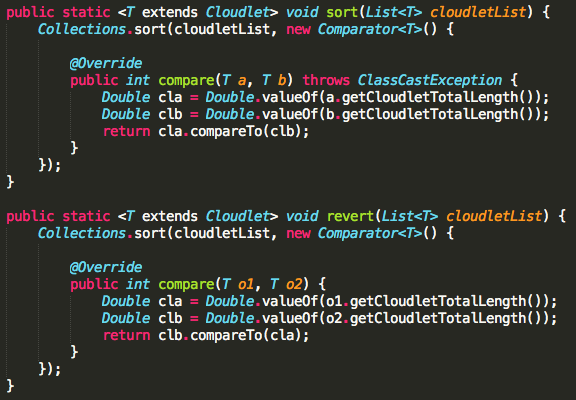
\includegraphics[scale=0.5]{media/ordenamientos}
	\caption{\textit{Algoritmos de Ordenamientos}. Fuente: Elaboración propia}
	\label{fig:sortRevert}
\end{figure}

%ver la seccion anexo